\section{Demystifying Test-Time Scaling in AI Agents}
\label{sect:char_implication}

We now explore the diverse design space of AI agents and examine their test-time scaling behavior to understand the trade-offs between model accuracy and cost. We evaluated accuracy following the official evaluation protocol of each benchmark. For HotpotQA and MATH, we report exact match accuracy, allowing minor formatting variations (e.g., equivalent mathematical expressions) in MATH. For WebShop, we use the task-specific score defined in the benchmark. For HumanEval, accuracy denotes the proportion of tasks that successfully pass all unit tests. To assess each design point, we used a benchmark of 50 sample questions and measured the average accuracy and the computation cost for each.

\subsection{Analyzing Cost-Efficiency Across AI Agent Design Spaces}
\label{sect:char_design_space}

Deploying AI agents in practical settings requires careful configuration of agentic system parameters. These design choices significantly affect not only the agent’s task success rate but also the overall cost of operating such systems. In this section, we quantify how different parameter configurations in AI agents influence both accuracy and cost-efficiency.

\begin{figure}[t!] \centering
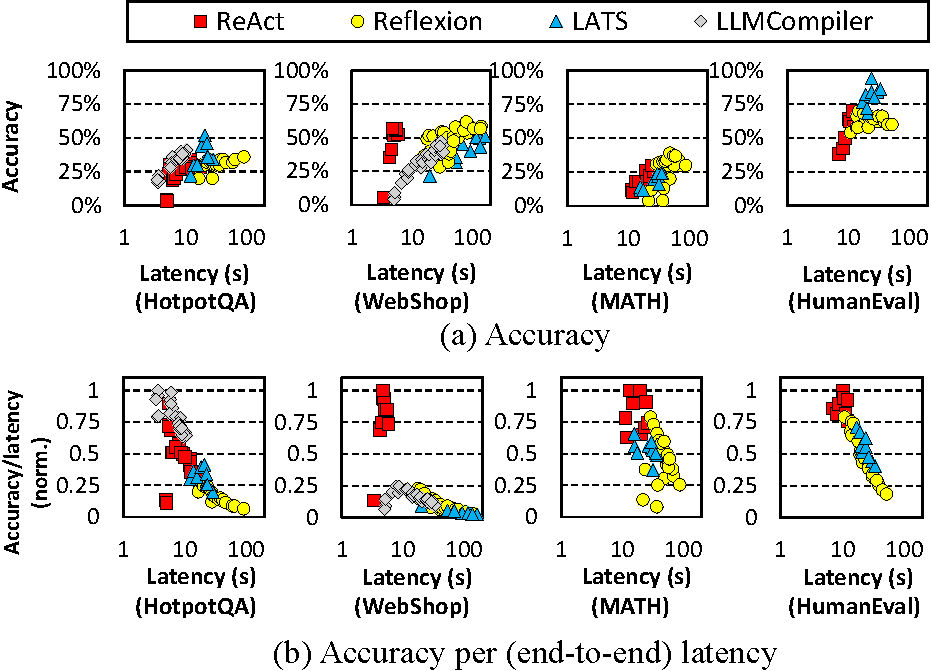
\includegraphics[width=0.48\textwidth]{./fig/pareto}
\vspace{-0.4em}
\caption{
Accuracy and cost-efficiency of AI agent design points. (a) Accuracy vs. latency and (b) Accuracy per latency, illustrating how efficiently each configuration translates cost into task performance.
}
\label{fig:pareto_compute_efficiency}
\end{figure}

\textbf{Pareto analysis of accuracy and cost across AI agent designs.} \fig{fig:pareto_compute_efficiency} presents the trade-off between accuracy and cost across various AI agent configurations. Each point corresponds to a specific design variant, such as changes to the number of few-shot examples or maximum iteration limits.


\fig{fig:pareto_compute_efficiency}(a) shows the trade-off between accuracy and latency. ReAct demonstrates strong compute efficiency across all benchmarks, achieving moderate accuracy with consistently low latency. Reflexion builds on ReAct by introducing reflection steps guided by internal or external rewards. This approach yields modest accuracy improvements but significantly increases latency. LATS extends Reflexion with a tree-based reasoning approach that explores multiple candidate branches at each step. While this leads to higher accuracy, it also introduces substantial computational overhead due to the expansion of reasoning paths. LLMCompiler, with its planning-based architecture, outperforms ReAct on tasks like HotpotQA in both accuracy and cost-efficiency, thanks to its ability to generate and execute structured plans in parallel. However, in tasks such as WebShop—where tool usage involves high interdependencies (e.g., searching or clicking on a webpage)—its DAG-style planning results in unnecessary tool invocations, leading to lower efficiency than ReAct.



\fig{fig:pareto_compute_efficiency}(b) illustrates the cost-efficiency of various agent configurations. We define cost-efficiency as the ratio of accuracy to cost, where cost is measured as end-to-end latency. This metric reflects how effectively each configuration translates compute resources into task accuracy\footnote{Using FLOPs as a proxy for cost (``accuracy per FLOP'') yielded similar qualitative conclusions, so we omit those results for brevity.}. Across all agents and workloads, we observe a consistent pattern: \emph{as computation cost increases, accuracy improves, but with diminishing returns}. This underscores the importance of designing AI agent serving systems that find configurations on (or near) the Pareto frontier, optimally balancing model accuracy against deployment cost rather than optimizing solely for accuracy.

\textbf{Tuning Iteration and Prompting for Cost-Efficient Agent Behavior.}
To better understand the accuracy–cost trade-offs in AI agent design, we analyze how two key parameters in AI agent designs affect model performance: the maximum iteration budget and the number of few-shot examples.

\begin{figure}[t!] \centering
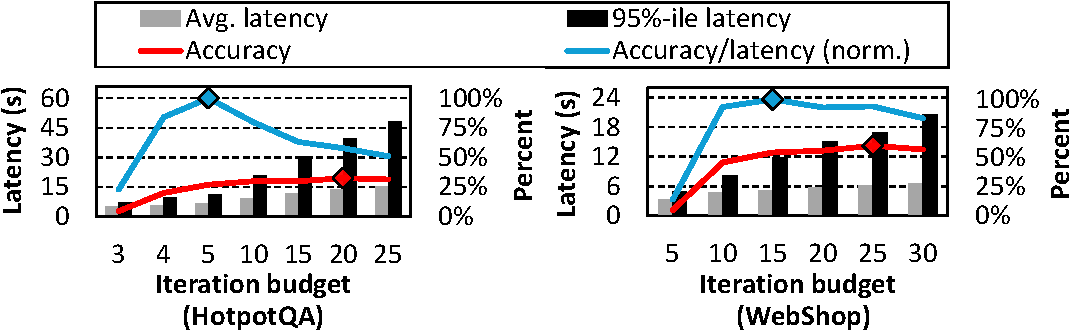
\includegraphics[width=0.48\textwidth]{./fig/design_space_iteration.pdf}
\vspace{-0.4em}
\caption{
End-to-end latency and accuracy trends under iteration budget constraints in ReAct. 
Markers indicate the points of maximum accuracy (red diamond) and peak cost-efficiency (blue diamond), as measured by accuracy-to-latency ratio.
}
\label{fig:design_space_iteration}
\vspace{-0.8em}
\end{figure}

\fig{fig:design_space_iteration} shows how varying the iteration budget impacts average latency, 95th percentile latency, and accuracy. The iteration budget controls how many reasoning steps and tool invocations the agent is allowed per query. As this budget increases, agents can perform deeper reasoning, which initially improves accuracy. However, both accuracy and average latency eventually saturate, while the 95th percentile latency continues to increase linearly. This rising tail latency is driven by a small set of outlier tasks that consume the full iteration budget. These outliers degrade cost-efficiency by contributing disproportionately to total compute usage without yielding substantial accuracy gains. The widening latency distribution also reduces predictability, which is especially problematic for latency-sensitive deployments. Therefore, iteration limits should be tuned not only for performance but also for latency consistency and operational stability.


\begin{figure}[t!] \centering
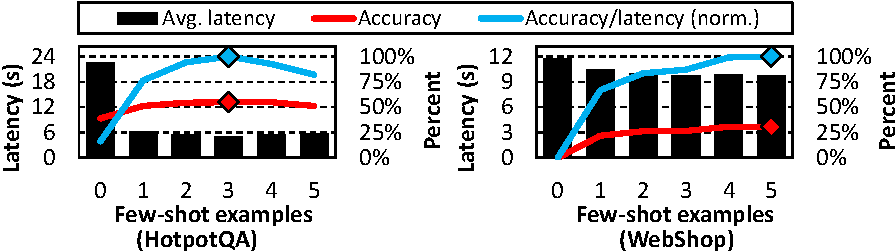
\includegraphics[width=0.48\textwidth]{./fig/design_space_fewshot_latency.pdf}
\vspace{-0.4em}
\caption{
End-to-end latency and accuracy trends with varying numbers of few-shot examples in ReAct. 
Markers indicate the configuration with the highest accuracy (red diamond) and the peak cost-efficiency (blue diamond), based on normalized accuracy-to-latency ratio.
}
\label{fig:design_space_fewshot_latency}
\end{figure}

\fig{fig:design_space_fewshot_latency} shows how varying the number of few-shot examples in the prompt affects latency and accuracy. Initially, adding examples substantially improves accuracy, as agents gain better task understanding. However, beyond a certain point, the benefit diminishes—and in some cases, accuracy declines due to prompt length exceeding the model’s optimal processing range. Interestingly, average latency decreases as more examples are added. This counterintuitive result arises because good examples help agents solve tasks in fewer steps, offsetting the cost of longer prompts. Thus, while longer prompts marginally increase per-token processing time, the reduction in overall reasoning steps often leads to net latency savings. In summary, a small number of carefully chosen examples can improve both accuracy and efficiency, while excessive prompting may lead to diminishing returns.

To identify optimal configurations, we highlight the point at which the accuracy-to-latency ratio is maximized (denoted by blue markers in \fig{fig:design_space_iteration} and \fig{fig:design_space_fewshot_latency}). This point represents the most cost-effective trade-off between model accuracy and response time. Such metrics provide a practical guideline for setting iteration budgets and few-shot prompting under latency or compute constraints.


\subsection{Test-Time Scaling of AI Agents}
\label{sect:char_scaling}

AI agents can dynamically scale their reasoning at test time by adjusting the number of reasoning steps based on task difficulty. This flexibility helps improve performance on complex problems, but it also introduces significant variation in computation cost. Designing systems that are both accurate and efficient requires a deeper understanding of how inference behavior evolves as compute usage increases.

\begin{figure}[t!] \centering
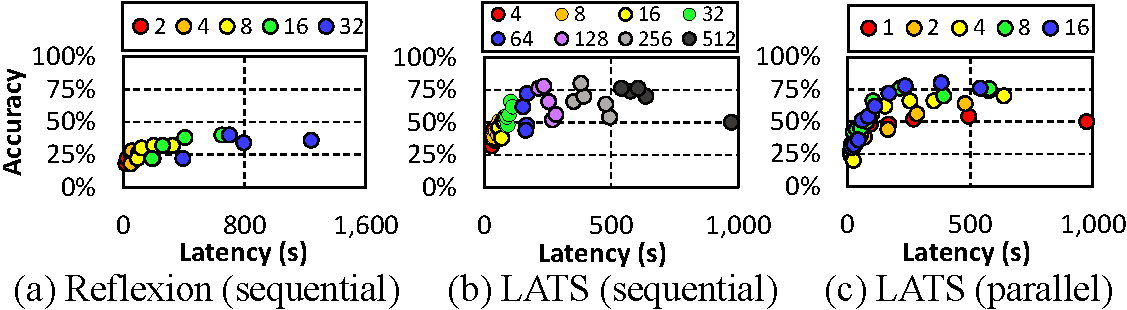
\includegraphics[width=0.48\textwidth]{./fig/test_time_scaling}
\vspace{-0.4em}
\caption{
Accuracy-latency trade-offs with sequential, parallel scaling on HotpotQA.
Legends denote the scaling level: maximum reflection steps in (a, b), and number of child nodes per expansion in (c). 
}
\label{fig:test_time_scaling}
\vspace{-0.8em}
\end{figure}

\textbf{Sequential vs. parallel reasoning at test time.}
We investigate the effect of two key forms of test-time scaling for AI agents: \emph{sequential} and \emph{parallel}. In \emph{sequential scaling}, the agent gradually increases its reasoning steps over time, allowing for deeper introspection. This is typical of agents like Reflexion and LATS, where the number of reflection steps can be adjusted dynamically. In contrast, \emph{parallel scaling} issues multiple reasoning branches simultaneously, commonly through parallel LLM calls, to explore diverse solution paths. LATS uses this approach by spawning multiple child nodes during each tree expansion step.

\fig{fig:test_time_scaling}(a) and (b) show the accuracy–latency trade-offs for Reflexion and LATS under sequential scaling. Both methods improve in accuracy with more reflection steps, but with diminishing returns. For example, in Reflexion, increasing latency from 16.9s to 25.6s yields a 4\% accuracy gain. However, achieving the same model accuracy improvement from a later point (56.0s) requires a much larger increase in latency (269.5s), a 31$\times$ higher cost for the same marginal gain.

On the other hand, parallel scaling exhibits a different trade-off. \fig{fig:test_time_scaling}(c) highlights the behavior under parallel scaling in LATS. Increasing the number of child nodes from 1 to 16 improves accuracy by 14.4 percentage points while simultaneously \emph{reducing} latency by 196.3s on average. This is because evaluating multiple reasoning paths in parallel helps the agent converge on high-quality answers more quickly. However, this comes at the cost of issuing more concurrent LLM requests, which increases memory pressure and may limit scalability in multi-tenant or resource-constrained environments.

These results suggest that AI agent configurations should align with system constraints such as latency budgets and available compute resources. Parallel scaling is effective for latency-sensitive workloads, as it allows the agent to explore multiple reasoning paths at once and reach better answers faster. However, it increases resource usage due to the large number of concurrent LLM calls.
In contrast, sequential scaling is better suited for resource-constrained environments. This approach avoids concurrent LLM calls, lowering peak resource demand, but incurs higher latency from step-by-step reasoning.

\begin{figure}[t!] \centering
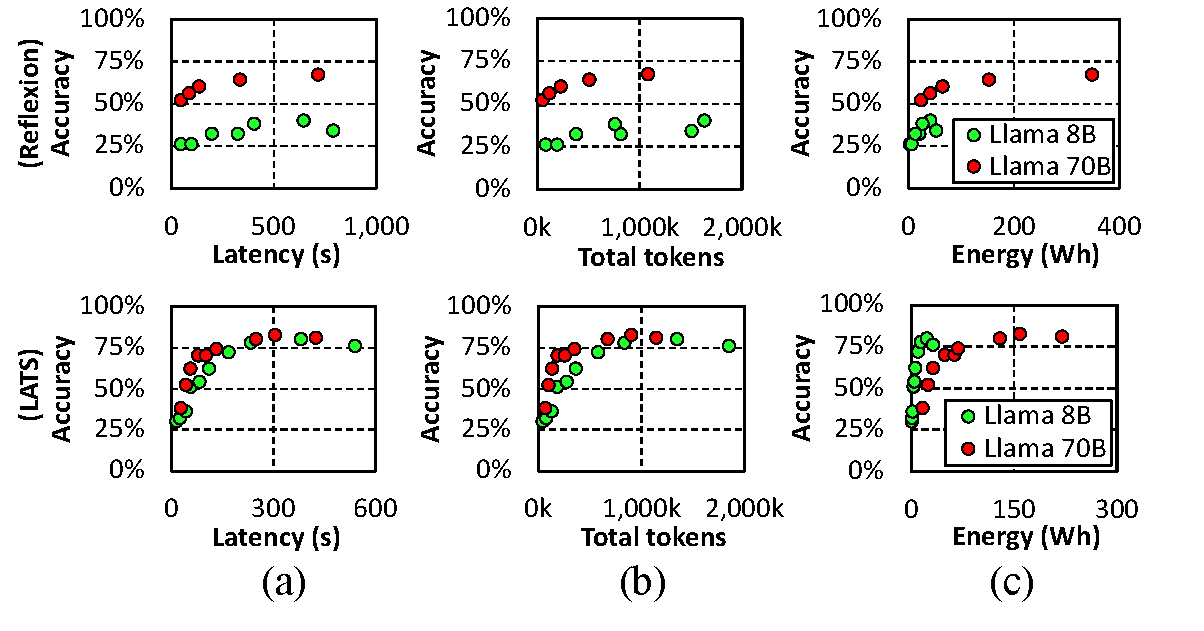
\includegraphics[width=0.48\textwidth]{./fig/test_time_scaling_models}
\vspace{-0.4em}
\caption{
Accuracy–cost trade-offs under test-time scaling across two model sizes (Llama-3.1-Instruct 8B and 70B) on HotpotQA. 
(a)–(c) compare Reflexion (top row) and LATS (bottom row) across latency, token usage, and energy consumption. 
While 70B achieves higher accuracy with fewer steps, the 8B model when paired with parallel scaling can approach 70B performance with lower energy cost. 
Each point denotes a different level of test-time reasoning.}
\label{fig:test_time_scaling_models}
\vspace{-1.0em}
\end{figure}

\textbf{Model size effects on test-time scaling.}
We further analyze how model size affects the accuracy–cost trade-offs under different test-time scaling strategies.

\fig{fig:test_time_scaling_models}(a) shows that both the 8B and 70B Llama-3.1-Instruct~\cite{llama_3.1_8b_instruct,llama_3.1_70b_instruct} models eventually reach saturation in accuracy, but they differ in how quickly they reach this point. The 70B model achieves high accuracy with relatively low latency, whereas the 8B model requires much longer inference times to reach similar performance. This trend is echoed in \fig{fig:test_time_scaling_models}(b), which plots total token usage. The 8B model consumes significantly more tokens at high-accuracy settings, indicating that it needs more reasoning iterations to match the 70B model's performance. However, as shown in \fig{fig:test_time_scaling_models}(c), the 8B model is substantially more energy-efficient. While the 70B model relies on 8 A100 GPUs, the 8B model runs on just one, resulting in lower total energy consumption per request, even when requiring more reasoning steps to be involved.

Interestingly, the performance gap between models can be partially closed with effective scaling strategies. Reflexion (which uses sequential scaling) shows limited accuracy on the 8B model. But with LATS and parallel scaling, the 8B model achieves near-70B performance by exploring multiple paths and selecting the best one. This shows that a test-time strategy can play a compensatory role in low-resource settings.



\section{AI Infrastructure Implications}
\label{sect:ai_infra}

In this section, we analyze the system-level impact of agentic test-time scaling by quantifying the GPU energy consumption and datacenter-wide power demands of AI agents relative to conventional single-turn LLM inference. Following the methodology in \sect{sect:char_scaling}, this section utilizes  Reflexion and LATS as representative AI agents that employ sequential and parallel scaling, respectively. Reflexion and LATS design points were selected based on the highest-accuracy configurations in \fig{fig:test_time_scaling_models}. Llama-3.1-Instruct 8B and 70B models are used as backend LLMs and ShareGPT serves as the baseline for conventional single-turn inference.

\textbf{GPU energy consumption.} 
Reflexion consumes 41.53 Wh and 348.41 Wh per query when using Llama-3.1-Instruct 8B and 70B as backend LLMs, whereas LATS consumes 22.76 Wh and 158.48 Wh (\tab{tab:test_time_scaling_cost}). By contrast, a conventional single-turn LLM inference (ShareGPT) requires only 0.32 Wh (8B) and 2.55 Wh (70B) per query. These figures correspond to a 62.1$\times$–136.5$\times$ increase in GPU energy per query under agent-based test-time scaling (vs. single-turn LLM inference).

Based on recent estimates, ChatGPT serves roughly 500 million to 1.27 billion weekly active users (WAU)~\cite{chatgpt_wau_500M,similarweb_chatgpt_2025,demandsage_chatgpt_stats,forbes_chatgpt_1b_2025}, which corresponds to approximately 71.4 million to 181.4 million daily active users (DAU). Assuming the conservative estimate of 71.4 million DAU and that each user submits just a ``single'' agentic query per day, Reflexion’s daily GPU energy consumption would be approximately 2.97~GWh for the 8B model and 24.89~GWh for the 70B model. Although our analysis does not account for LLM request batching~\cite{orca,vllm}, which can amortize execution overheads, the estimate remains conservative for three reasons: (1) it represents a lower-bound based on the conservative DAU estimate of 71.4 million and assumes just one query per user, despite accelerating adoption and increasing user demand, (2) it includes only GPU energy, omitting overheads from CPU, memory, networking, storage, and cooling, and (3) even the larger 70B model considered in our study is orders of magnitude smaller than today's large-scale LLMs, which now reach hundreds of billions to trillions of parameters~\cite{meta2025llama4,moonshot2025kimi,deepseekai2025deepseekr1,felloai2024gemini15}.

Even under these modest assumptions, the projected demand rivals the daily electricity consumption of Seattle and its surrounding area (24.8 GWh)~\cite{seattle_city_light_report}. As AI agents become increasingly embedded in everyday applications, their query volume could approach, or exceed, that of traditional search engines. For instance, Google Search processes over 13.7 billion queries per day~\cite{google_statistics}, roughly 192$\times$ the 71.4 million agentic queries assumed above. If this growth in user base and usage persists, AI infrastructure demand could rise dramatically, potentially exceeding sustainable limits and underscoring the significant challenges posed by test-time scaling.


\begin{scriptsize}
\begin{table}[t]
\centering
\caption{
Accuracy, latency, and  GPU energy consumption when servicing a single agent request on HotpotQA. Numbers in parentheses indicate the relative increase over ShareGPT (the conventional single-turn inference). 
}
\begin{tabular}{cc|cccccc}
\hline
& & \multicolumn{2}{c}{\makecell[c]{\textbf{Accuracy} \\ \textbf{(\%)}}} & \multicolumn{2}{c}{\makecell[c]{\textbf{Latency} \\ \textbf{(seconds)}}} & \multicolumn{2}{c}{\makecell[c]{\textbf{Energy} \\ \textbf{(Wh/query)}}}\\
\hline
\hline
\multirow{3}{*}{8B} 
    & \textbf{ShareGPT}  & \multicolumn{2}{c}{--} & \multicolumn{2}{c}{4.23 (1×)} & \multicolumn{2}{c}{0.32 (1×)}\\
    & \textbf{Reflexion} & \multicolumn{2}{c}{38} & \multicolumn{2}{c}{649.34 (153.7×)} & \multicolumn{2}{c}{41.53 (130.9×)}\\
    & \textbf{LATS}      & \multicolumn{2}{c}{80} & \multicolumn{2}{c}{380.90 (90.1×)} & \multicolumn{2}{c}{22.76 (71.7×)}\\ \hline
\multirow{3}{*}{70B} 
    & \textbf{ShareGPT}  & \multicolumn{2}{c}{--} & \multicolumn{2}{c}{6.40 (1×)} & \multicolumn{2}{c}{2.55 (1×)}\\
    & \textbf{Reflexion} & \multicolumn{2}{c}{67} & \multicolumn{2}{c}{720.00 (112.6×)} & \multicolumn{2}{c}{348.41 (136.5×)}\\
    & \textbf{LATS}      & \multicolumn{2}{c}{82} & \multicolumn{2}{c}{305.67 (47.8×)} & \multicolumn{2}{c}{158.48 (62.1×)}\\
\hline
\end{tabular}
\label{tab:test_time_scaling_cost}
\end{table}
\end{scriptsize}

\begin{scriptsize}
\begin{table}[t]
\centering
\caption{
Datacenter-wide power demand under current and future traffic scenarios (71.4 Million and 13.7 Billion Queries/day), assuming the HotpotQA benchmark.
}
\begin{tabular}{cc|cccccc}
\hline
& & \multicolumn{3}{c}{\makecell[c]{\textbf{Power @ 71.4 Million} \\ \textbf{Queries/day (Watts})}} & \multicolumn{3}{c}{\makecell[c]{\textbf{Power @ 13.7 Billion} \\ \textbf{Queries/day (Watts})}}\\
\hline
\hline
\multirow{3}{*}{8B} 
    & \textbf{ShareGPT} & \multicolumn{3}{c}{1.0 M} & \multicolumn{3}{c}{182.7 M}\\
    & \textbf{Reflexion} & \multicolumn{3}{c}{123.6 M} & \multicolumn{3}{c}{23.7 G}\\
    & \textbf{LATS}      & \multicolumn{3}{c}{67.7 M} & \multicolumn{3}{c}{13.0 G}\\ \hline
\multirow{3}{*}{70B} 
    & \textbf{ShareGPT}  & \multicolumn{3}{c}{7.6 M} & \multicolumn{3}{c}{1.5 G}\\
    & \textbf{Reflexion} & \multicolumn{3}{c}{1.0 G} & \multicolumn{3}{c}{198.9 G}\\
    & \textbf{LATS}      & \multicolumn{3}{c}{471.5 M} & \multicolumn{3}{c}{90.5 G}\\
\hline
\end{tabular}
\label{tab:power_demand}
% \vspace{-1.6em}
\end{table}
\end{scriptsize}

\textbf{Datacenter-wide power demands.} We now move on to estimating the datacenter-wide power requirements to sustain the aforementioned AI service demands, assuming today's (ChatGPT's 71.4 million queries per day, assuming the conservative ChatGPT DAU estimate and one agentic query per user) and tomorrow's (Google search's 13.7 billion queries per day) AI traffic. \tab{tab:power_demand} translates the per-query GPU energy consumption numbers into datacenter-level power requirements, computed by $P=(\text{Wh/query})\times ((\text{Queries/Day})/(24\text{ hours}))$. Under today’s 71.4 million DAU load, single-turn ShareGPT (70B) requires roughly 7.6 MW, well within the tens-of-megawatts envelope typical of modern datacenters~\cite{hyperscale_datacenter,xAI_collosus}. However, assuming similar traffic levels for AI agents, even the lighter 8B-based agents demand 67.7–123.6 MW, comparable to the power draw of a mid-sized U.S.\ city, while 70B-based agents approach 1 GW, nearly three orders of magnitude higher than the single-turn LLM baseline. Strikingly, this gigawatt-scale power requirement aligns with the announced budget for OpenAI’s multi-gigawatt Stargate facility~\cite{openai_stargate}, which is intended to support \emph{future} AI model deployments. Yet, our analysis suggests that such infrastructure may already be necessary to support agentic systems under today’s traffic levels. Overall, our estimates indicate that even modest user traffic (on the order of tens of millions of queries per day) becomes gigawatt-scale once per-query energy exceeds \(\sim\)100 Wh, a threshold representative of current agentic workloads.

If we were to scale the same per-query figures to Google’s 13.7 billion daily searches, the power numbers would raise single-turn ShareGPT (70B) to 1.5 GW and Reflexion (70B) to nearly 200 GW, far beyond any announced datacenter project (e.g., Meta's recently announced 5 GW AI datacenter Hyperion is scheduled for deployment in 2030~\cite{meta_hyperion_prometheus}) and exceeding the power budgets of many national grids. To put this number into perspective, a 200 GW is almost half of the \emph{entire} U.S. grid's average load (which amounts to 4,178$\times10^3$\text{ GWh}/(365$\times$24$\text{ hours})$$=$ 476.9$\text{ GW}$~\cite{us_grid_load}), a scale usually discussed only for nation-wide decarbonization plans, not for a single industry or technology, one that fundamentally reshapes generation, transmission, and sustainability planning.

{\bf Sustainability challenges of agentic test-time scaling. } Collectively, our findings show that AI agent performance does not scale proportionally with the associated compute, energy, and power costs. Once accuracy saturates, additional test-time scaling yields diminishing returns while imposing substantial system-level burdens. This cost inefficiency is not merely theoretical; it poses concrete constraints on real-world deployments. For instance, OpenAI’s Deep Research~\cite{deep_research}, designed for complex multi-step reasoning, can take up to 30 minutes per request~\cite{deep_research_faq}. To keep infrastructure costs manageable, OpenAI limits usage to 25 runs every 30 days for ChatGPT Plus users~\cite{deep_research_faq}. These limits highlight the financial and computational challenges of sustaining AI systems that rely heavily on intensive test-time computation.

Based on these findings, we argue that building scalable and sustainable AI agents requires moving away from unconstrained test-time scaling. Instead, AI agents should be designed with compute-aware agentic workflows that deliver strong performance through efficient inference, rather than single-handedly relying on extended reasoning depth. 



